\section{Theorie}
\label{sec:Theorie}

\subsection{Funktionsweise}
    Bei einer Brückenschaltung wird die Potentialdifferenz von zwei 
    parallelen Leitern, die jeweils mit unterschiedlichen Widerständen 
    versehen sind, gemessen.\\
    Typischerweise besteht die Schaltung also aus zwei parallel geschalteten 
    Widerstandsfolgen, wie das Schaltbild %\ref{fig:schalt_generell}
    zeigt.\\

    \noindent Zur Berechnung der sogenannten Brückenspannung $U_{\text{Br}}$
    werden die Kirchhoffschen Gesetze verwendet.\\
    \begin{enumerate}
        \item Knotenregel: Treffen mehrere Ströme aufeinander, ist die Gesamtsumme
        aller Ströme gleich null, wobei abfließende Ströme ein negatives Vorzeichen
        haben.\\
        \begin{equation}
            \sum_k I_k = 0
            \label{eqn:knoten}
        \end{equation}
        \item Maschenregel: In dem geschlossenen Stromkreisen ist die Summer
        aller elektromotorischen Kräfter gleich der Summer aller Stromstärken 
        multipliziert mit den Widerständen. Auch hier sind eine Ströme negativ 
        zu werten; diejenigen, die entgegen dem Uhrzeigersinn laufen.\\
        \begin{equation}
            \sum_k E_k = \sum_k I_k R_k
            \label{eqn:maschen}
        \end{equation}
    \end{enumerate}

    \noindent Im Fall der allgemeinen Brückenschaltung folgt aus \eqref{eqn:knoten}
    und \eqref{eqn:maschen} die Bedingung 
    \begin{equation}
        R_1 R_4 = R_2 R_3
        \label{eqn:abgleich}
    \end{equation}
    Ist sie erfüllt, spricht man von einer abgeglichenen Brücke. \\
    Oftmals werden auch Kapazitäten und Induktivitäten in eine Brückenschaltung eingebaut,
    in diesem Fall werden die Widerstände als komplexe Zahlen aufgefasst; es gelten
    \begin{align*}
        Z_C = - \frac{i}{\omega}\\
        Z_L = i \omega L\\
        Z_R = R
    \end{align*}
    für die Impedanzen (komplexen Widerstände) von Kapazität $C$, Induktivität $L$ und ohm'schem
    Widerstand $R$.

\subsection{Wheatonsche Brücke}
    Eine Wheatonschene Brückenschaltung ist aufgebaut wie in Abbildung %\ref{fig:wheaton}
    dargestellt. Sie besteht ausschließlich aus ohmschen Widerständen und kann genutzt werden,
    um den Widerstand $R_x$ zu berechnen. Für ihn gilt
    \begin{equation}
        R_x = R_2 \frac{R_3}{R_4}
    \end{equation}

    \begin{figure}
        \centering
        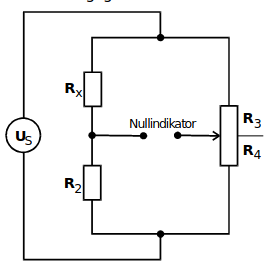
\includegraphics[width=\textwidth]{wheaton.png}
        \caption{Schaltbild der Wheatonschen Brücke.}
        \label{fig:kap}
    \end{figure}
        

\subsection{Kapazitätsmessbrücke}
    Durch die bei Kondensatoren anfallenden thermischen Verluste kommt zur Kapazität noch ein ohm'scher Widerstand hinzu, sodass
    \begin{equation}
        Z_{C,\text{real}} = R - \frac{i}{\omega C} .
    \end{equation}
    Im Gegensatz zur Wheatonschen Brücke müssen also zwei Unbekannte bestimmt werden, $C_x$ und $R_x$, daher ist ein weiterer 
    veränderlicher Widerstand eingebaut. Mit ihm wird die Phasenverschiebung kompensiert, die durch $R_x$ hinzu kommt.\\
    $R_x$ kann auf die gleiche Weise wie in der Wheatonschen Brückenschaltung ermittelt werden (mit dem einzigen Unterschied,
    dass $R_2$ nun ein veränderlicher Widerstand ist), für $C_x$ gilt
    \begin{equation}
        C_x = C_2 \frac{R_4}{R_3}
    \end{equation}

    \begin{figure}
        \centering
        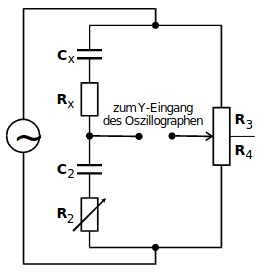
\includegraphics[width=\textwidth]{kap.png}
        \caption{Schaltbild Kapazitätsmessbrücke.}
        \label{fig:kap}
    \end{figure}

\subsection{Induktivitätsmessbrücke}
    Auch bei einer Induktivität muss in der Realität der thermische Verlust betrachtet werden. Auf dieselbe Weise wie bei der Kapazität 
    wird das Schaltbild zu einem ERsatzschaltbild mit ohmschem Widerstand erweitert.\\
    Es gilt für die Impedanz der Induktivität
    \begin{equation}
        Z_{L, \text{real}} = R + i \omega L.
    \end{equation}
    Die Induktivitätsmessbrücke funktioniert daher genau wie die Kapazitätsmessbrücke, abgesehen davon, dass anstatt einem Kondensator $C_2$ 
    eine Induktivität verbaut wird. Die Abgleichbedingungen werden zu 
    \begin{align}
        R_x = R_2 \frac{R_3}{R_4}\\
        L_x = L_2 \frac{R_3}{R_4} .
    \end{align} 

    \begin{figure}
        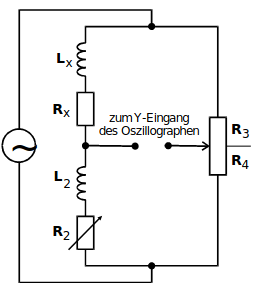
\includegraphics[width=\textwidth]{ind.png}
        \centering
        \caption{Schaltbild der Induktivitätsrücke.}
        \label{fig:ind}
    \end{figure}

\subsection{Maxwell-Brücke}
    Eine andere Möglichkeit, die Induktivität zu messen, besteht in der Maxwell-Brücke. Sie verwendet zwei veränderliche Widerstände zum Abgleichen,
    von denen einer mit einem Kondensator parallel geschaltet ist wie in \ref{fig:maxwell} zu sehen.\\
    Die Abgleichbedingung wird zu 
    \begin{align}
        R_x = \frac{R_2 R_3}{R_4}\\
        L_x = R_2 R_3 C_4 .
    \end{align}
    In der Realität ist die Maxwell-Brücke für eine bestimmten Frequenzbereich optimal zur Messung geeignet, auch wenn die Abgleichbedingung unabhängig
    von der Spannung ist. Dies liegt an Streukapazitäten in der Verdrahtung der Bauteile, die besonders bei hohen Frequenzen nicht zu vernachlässigen sind, 
    und an den langen Einschwingvorgängen, die bei niedrigen Frequenzen problematisch werden können.

    \begin{figure}
        \centering
        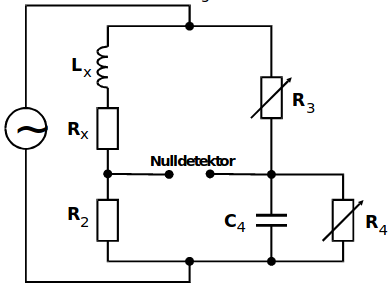
\includegraphics[width=\textwidth]{maxwell.png}
        \caption{Schaltbild der Maxwell-Brücke.}
        \label{fig:maxwell}
    \end{figure}

\subsection{Wien-Robinson-Brücke}
    Mit einem anderen Prinzip funktioniert die Wien-Robinson-Brücke. Wie in Abbildung \ref{fig:wien} zu sehen benötigt sie keinerlei Abgleichelemente,
    stattdessen ist die Frequenz für den Abgleich essentiell. Solche Brückenschaltungen werden daher als frequenzabhängig bezeichnet.\\
    Grob lässt sich die Schaltung in vier Zweige aufteilen, deren Impedanzen lassen sich schreiben als
    \begin{align}
        Z_1 = 2 R'\\
        Z_2 = R'\\
        Z_3 = R + \frac{1}{i \omega C}\\
        Z_4 = \frac{R}{1 + i \omega R C}
    \end{align}
    Aus diesen Verhältnissen folgt naus \eqref{eqn:maschen} für das Verhältnis aus Brückenspannung $U_{\text{Br}}$ und Speisespannung $U_{\text{Sp}}$
    \begin{equation}
        \left| \frac{U_{\text{Br}}}{U_{\text{Sp}}} \right|^2 = \frac{1}{9} \cdot \frac{\left(\omega^2 R^2 C^2 - 1\right)^2}{\left(1 - \omega^2 R^2 C^2\right)^2 + 9 \omega^2 R^2 C^2}
    \end{equation}
    Dies kann null werden für $\omega_0 = \frac{1}{RC}$. Mit der Substitution $\Omega = \frac{\omega}{\omega_0}$ wird die obige Gleichung in eine elegantere 
    Form gebracht
    \begin{equation}
        \left| \frac{U_{\text{Br}}}{U_{\text{Sp}}} \right|^2 = \frac{1}{9} \cdot \frac{\left(\Omega^2 - 1\right)^2}{\left(1 - \Omega^2\right)^2 + 9 \Omega^2}
    \end{equation}
    was einem elektrischen Filter für Frequenzen in der Nähe von und gleich $\omega_0$ gleichkommt.

    \begin{figure}
        \centering
        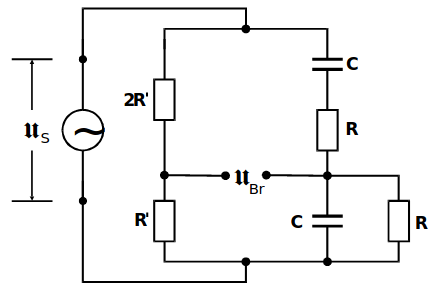
\includegraphics[width=\textwidth]{wien.png}
        \caption{Schaltbild der Wien-Robinson-Brücke.}
        \label{fig:wien}
    \end{figure}